
\chapter{\lsystem}

History of \lsystem was mentioned in introduction.
This chapter will describe \lsystem formally.
First we will describe \lsystem in general and then we describe some special features of \lsystem.


\section{Formal definition of \lsystem}

\lsystem $L$ is formally triplet $L = (\Sigma, \omega, R)$, where

\begin{itemize*}
	\item $\Sigma$ is alphabet, non-empty set of symbols ($\Sigma^{*}$ is set of all words over the alphabet $\Sigma$, $\Sigma^{+}$ is set of all non-empty words over the alphabet $\Sigma$),
	\item $\omega \in \Sigma^{+}$ is axiom (also called seed), word defining the initial state of the \lsystem,
	\item $R \subset \Sigma \times \Sigma^{*}$ is finite set of rewrite rules (production rules), rewrite rule defining rewriting symbol $s \in \Sigma$ to word $w \in \Sigma^{*}$ is written as $s \rightarrow w$.
\end{itemize*}

For any symbol $s \in \Sigma$ which does not appear on the left hand side of any rewrite rule in $R$, the identity rewrite rule $s \rightarrow s$ is assumed.
These symbols are called constants or terminals.

Formal definition of \lsystem is similar to deterministic context-free grammar but there are few differences.
In grammar we distinguishes terminal and non-terminal symbols, but in \lsystems we do not define them explicitly (we define identity rewrite rule for terminal symbols in \lsystems).
Next difference is in initial string.
In grammar we have only one symbol as initial state but \lsystem allows non-empty word.
The biggest difference is in rewriting principles which is described is following section.


\subsection{Rewriting principles of \lsystem}

\lsystem is developing in iterations.
Rewrite rules of the \lsystem grammar are applied iteratively starting from the initial state.
In each iteration is all symbols are rewritten.
This is possible because all symbols are on left side of some rewrite rule (if symbol would not be on left side of some rewrite rule, identity rule will be defined).
There is only one way how to rewrite iteration thus rewriting is deterministic.


Rewriting of symbols is parallel (all symbols are rewritten at once).
This means that if some symbol is rewritten, resulting symbols are not rewritten again in the same iteration.
[Example]

Described rewriting mechanics distinguishes \lsystem and formal grammar.
In grammar there is not mandatory to rewrite all possible symbols.
Thus, \lsystems are strict subsets of languages.

\lsystem in figure \ref{fig:rrExample} produces strings shown in table \ref{fig:rrExampleResult}.
\lsystem starts with axiom $A$ and two rewrite rules $A \rightarrow B$ and $B \rightarrow A B$.
In first iteration axiom $A$ is rewritten by first rewrite rule to $B$.
In second iteration is $B$ rewritten with second rewrite rule to symbols $A B$.
In third iteration is first symbol $A$ rewritten to $B$ and second symbol $B$ rewritten to $A B$ which gives string $B A B$ ...

\begin{figure}[ht]
	\begin{Lsystem}
lsystem RewritingExample {
	set symbols axiom = A;
	set iterations = 6;
	set interpretEveryIteration = true;
	rewrite A to B;
	rewrite B to A B;
}
process all with SymbolPrinter;
	\end{Lsystem}
	\caption{Simple \lsystem as example of rewriting principles}
	\label{fig:rrExample}
\end{figure}

\begin{table}[ht]
	\centering
	\begin{tabular}{c l}
   		\toprule
   		Iteration & String of symbols \\
   		\midrule
		0 & A \\
		1 & B \\
		2 & A B \\
		3 & B A B \\
		4 & A B B A B \\
		5 & B A B A B B A B \\
		6 & A B B A B B A B A B B A B \\
		\bottomrule
	\end{tabular}
	\caption{Result of \lsystem from figure \ref{fig:rrExample}}
	\label{fig:rrExampleResult}
\end{table}

\lsystem in figure \ref{fig:rrExample} has also some interesting properties.
String of symbols in every iteration (expect the axiom) is suffix of string in following iteration.
Also count of symbols in iterations gives Fibonacci sequence\footnote{Fibonacci sequence is defined by following the recurrence relation $F_n = F_{n-1} + F_{n-2}$ where $F_0 = F_1 = 1$.} 1, 1, 2, 3, 5, 8, 13,~...

\subsection{Interpretation of \lsystem symbols}

Result of \lsystem rewriting is string of symbols, we can interpret symbols in any way we want.
Most common and the simplest interpretation of \lsystem symbols is interpret them as 2D graphics elements like lines or polygons.
The first who came with this type of interpretation was Przemyslaw Prusinkiewicz who interpreted \lsystem symbols with Logo-like turtle~\cite{Pru85}.
Logo is programming language that controls cybernetic turtle which is drawing on 2D canvas.
This can be easily extended into 3D.

Interpretation of symbols can arbitrary. [maybe write something more here]
%Symbols can be interpreted as music~\cite{HCJ99, Man06}.


\section{\lsystem features}

In this section we will describe extending features of \lsystem rewriting and interpreting system.
Some features may require extension of described formal definition of \lsystem but it will be omitted.


\subsection{Basic \lsystem}

\begin{wrapfigure}{r}{0.5\textwidth}
	\vspace{-40pt}
	\begin{center}
	\includegraphics[width=0.48\textwidth]{BasicLsystem}
	\end{center}
	\caption{Dragon curve}
	\label{fig:basicLsystem}
\end{wrapfigure}


\newcommand{\dzerolsystem}{\mbox{D0L-system}\xspace}
\newcommand{\dlsystem}{\mbox{dL-system}\xspace}

Basic \lsystem is called \dzerolsystem{}\footnote{\dzerolsystem is also called just \dlsystem~\cite{Zar04}}, \emph{D} stands for deterministic and \emph{0} means it is context-free.
Deterministic \lsystems have rewrite rules which have just one way how to rewrite symbol.
Because of rewriting principle which rewrites all symbols in each iteration the whole rewriting process is deterministic -- result depends only on axiom.

Figure \ref{fig:basicLsystem} shows Dragon curve generated by \dzerolsystem \ref{fig:basicLsystemSrc}.

\begin{figure}[ht]
	\begin{Lsystem}
lsystem DragonCurve {
	set symbols axiom = L;
	set iterations = 12;
	interpret R L as DrawForward(5);
	interpret + as TurnLeft(90);
	interpret - as TurnLeft(-90);
	rewrite L to L + R +;
	rewrite R to - L - R;
}

process all with SvgRenderer;
	\end{Lsystem}
	\caption{Basic \dzerolsystem for generation of Dragon curve (fig. \ref{fig:basicLsystem})}
	\label{fig:basicLsystemSrc}
\end{figure}


%\newpage
\subsection{Branching system}

\begin{wrapfigure}{r}{0.32\textwidth}
	\vspace{-50pt}
	\begin{center}
	\includegraphics[width=0.3\textwidth]{Branching}
	\end{center}
	\caption{Plant}
	\label{fig:branching}
\end{wrapfigure}

First and important extension to \lsystems is branching system.
This type of \lsystems are called Bracketed \lsystems\cite{PL91} but it is so fundamental feature that it is not explicitly mentioned.
It extends linear string of symbols to the tree structure.
Individual branches do not affect each other nor their root.
This allows to model plants more easily and create more complex models.

Branching is achieved by allowing saving and loading the state of \lsystem.
By state we mean state of interpretation like position, orientation, color or width.
Saving and loading operations can be assigned to any symbols but most common are brackets.

\begin{figure}[ht]
	\begin{Lsystem}
lsystem BranchingExample {
	set symbols axiom = X;
	set iterations = 7;
	set initialAngle = 90;
	interpret F(age) as DrawForward(2^age, age / 2);
	interpret + as TurnLeft(20);
	interpret - as TurnLeft(-20);
	interpret [ as StartBranch;
	interpret ] as EndBranch;
	rewrite F(age) to F(age + 1);
	rewrite X to F(1) [ + X ] F(1) [ - X ] + X;
}
process all with SvgRenderer;
	\end{Lsystem}
	\caption{Example of usage of branches to create plant-like model (fig. \ref{fig:branching})}
	\label{fig:branchingSrc}
\end{figure}



\subsection{Stochastic \lsystems}

All plants generated by same deterministic \lsystem are identical.
Forest made by trees which are identical looks artificial.
Stochastic \lsystems solves this problem.
Stochastic \lsystems are called 0L-systems where \emph{0} means they are context-free.

Randomization of model produced by \lsystem can be done in two places, in rewrite rules or in interpretation of symbols (or in both).
Randomization in interpretation can only change properties of interpreted symbols such as lengths of lines or turning angles, the topology of plant remains unchanged.
In contrast with rewrite rule randomization which can also change topology of model.
Rewrite rule randomization is done by defining more replacements for one rewrite rule.
Rewriting system will pick random replacement if rewrite rule is applied.
Each replacement can have different probability to be picked.

On figure \ref{fig:randComparison} are shown 3 models of plant generated by \lsystems.
First image \ref{fig:randComparisonNo} was generated without any randomization.
Second image \ref{fig:randComparisonInt} was generated with interpretation randomization of line lengths and angles.
For last image \ref{fig:randComparisonBoth} was also added topology randomization with rewrite rule randomization.
Source code for last image is shown in figure \ref{fig:randExample}.

\begin{figure}[ht]
	\centering
	\subfloat[No randomization]{
		\label{fig:randComparisonNo}
		\includegraphics[width=0.3\textwidth]{StochasticLsystemExample-NoStochasism}
	} ~
	\subfloat[Angles, lengths randomized]{
		\label{fig:randComparisonInt}
		\includegraphics[width=0.32\textwidth]{StochasticLsystemExample-InterpretationStochasism}
	} ~
	\subfloat[Also topology randomized]{
		~
		\label{fig:randComparisonBoth}
		\includegraphics[width=0.25\textwidth]{StochasticLsystemExample-BothStochasism}
		~
	}
	\caption{Comparison between non-randomized and randomized plant model}
	\label{fig:randComparison}
\end{figure}

\begin{figure}[ht]
	\begin{Lsystem}
lsystem StochasticLsystemExample {
	set symbols axiom = X;
	set initialAngle = 90;
	set iterations = 8;
	set randomSeed = 1036793868;

	interpret F(age) as DrawForward(1.8^age * random(0.5, 1.5), age / 2);
	interpret + as TurnLeft(45 + random(-20, 20));
	interpret - as TurnLeft(-45 + random(-20, 20));
	interpret [ as StartBranch;
	interpret ] as EndBranch;

	rewrite F(age) to F(age + 1);
	rewrite X
		to F(1) [ + X ] [ - X ] F(1) X  weight 4 or
		to F(1) [ + X ] F(1) X          weight 1 or
		to F(1) [ - X ] F(1) X          weight 1;
}
process all with SvgRenderer;
	\end{Lsystem}
	\caption{Example or stochastic \lsystems with randomized rewrite rules and interpretation}
	\label{fig:randExample}
\end{figure}

\begin{comment}
\subsection{Context rewriting}

\newcommand{\onelsystems}{\mbox{1L-systems}\xspace}
\newcommand{\twolsystems}{\mbox{2L-systems}\xspace}

Context sensitive rewrite rules allows to rewrite symbol depending on the context (symbols around it).
Formally there are two types of context sensitive L-systems, \onelsystems and \twolsystems.
Rewrite rules of \onelsystems check context only on one side (left or right) whereas rewrite rules of \twolsystems check context on both sides.
Since \onelsystems are just \twolsystems with one context empty we will consider context sensitive \lsystems as \twolsystems.

Context sensitive \lsystems can be used for simulating signal propagation in string of symbols.

\begin{figure}[ht]
	\begin{Lsystem}
lsystem RewritingExample {
	set symbols axiom = B A A A A A;
	set iterations = 6;
	set interpretEveryIteration = true;
	rewrite {B} A     to B;
	rewrite     B {A} to A;
}
process all with SymbolPrinter;
	\end{Lsystem}
	\caption{\lsystem simulating signal propagation}
	\label{fig:signalPropagarionSrc}
\end{figure}

\begin{table}[ht]
	\centering
	\begin{tabular}{c l}
   		\toprule
   		Iteration & String of symbols \\
   		\midrule
		0 & B A A A A A \\
		1 & A B A A A A \\
		2 & A A B A A A \\
		3 & A A A B A A \\
		4 & A A A A B A \\
		5 & A A A A A B \\
		6 & A A A A A A \\
		\bottomrule
	\end{tabular}
	\caption{Result of \lsystem from figure \ref{fig:signalPropagarionSrc}}
	\label{fig:signalPropagarion}
\end{table}

Context search in bracketed \lsystems is more difficult.
The context matching procedure is searching context with respect to following rules:
\begin{enumerate*}
	\item \label{enum:ctxRule1} two symbols are neighbors even if there are some branches between them,
	\item \label{enum:ctxRule2} left neighbor of first symbol in branch is symbol before branch,
	\item \label{enum:ctxRule3} last symbol in branch do not have right neighbor,
	\item \label{enum:ctxRule4} unmatched symbols at end of branch are ignored,
	\item \label{enum:ctxRule5} order of branches is insignificant.
\end{enumerate*}

These rules defines natural behavior of context between branches.
Table \ref{tbl:bracketCtxt} shows examples of context matching in bracketed \lsystems with references to according rules.

\begin{table}[ht]
	\centering
	\begin{tabular}{c c c p{128pt} c c}
   		\toprule
   		Left ctx. & Symbol & Right ctx. & Symbol string & Match & Rule\\
   		\midrule
		 & X & Y & A B \textbf{X} [ A [ B ] ] [ C ] \textbf{Y} & yes & \ref{enum:ctxRule1} \\
		 & X & Y & A B \textbf{X} [ Y B ] C Y & no &  \\
		 Y & X & & A B \textbf{Y} [ \textbf{X} A B ] C & yes & \ref{enum:ctxRule2} \\
		 Y & X & & A B \textbf{Y} [ [ \textbf{X} A ] B ] C & yes & \ref{enum:ctxRule2} \\
		 & X & Y & A [ B \textbf{X} ] Y & no & \ref{enum:ctxRule3} \\
		 & X & [ Y ] & A B \textbf{X} [ \textbf{Y} A B ] A  & yes & \ref{enum:ctxRule4} \\
		 & X & [ [ Y ] ] & A B \textbf{X} [ [ \textbf{Y} A B ] C ] & yes & \ref{enum:ctxRule4} \\
		 & X & [ Y ] & A B \textbf{X} [ A B ] [ \textbf{Y} ] A  & yes & \ref{enum:ctxRule5} \\
		 & X & [ Y ] [ Z ] & A B \textbf{X} [ \textbf{Z} ] [ \textbf{Y} ] A  & yes & \ref{enum:ctxRule5} \\
		\bottomrule
	\end{tabular}
	\caption{Examples of context matching in bracketed \lsystems}
	\label{tbl:bracketCtxt}
\end{table}

Context in bracketed \lsystems can be used for propagation of signals through tree structure.
There are two basic types of signals.
First is \emph{acropetal} signal which spreads from root to branches and second is \emph{basipetal} which spreads in other way i.e. from branches to root.
This can be used well in plant modeling.
Following figures shows context \lsystems for simulating acropetal (\ref{fig:acropetalSignal}) and basipetal (\ref{fig:basipetalSignal}) signals in static plant-like structure.
Segments with signal are marked bolder.

\begin{figure}[ht]
	\centering
	\subfloat{\includegraphics[height=100pt]{AcropetalSignal1}} ~
	\subfloat{\includegraphics[height=100pt]{AcropetalSignal2}} ~
	\subfloat{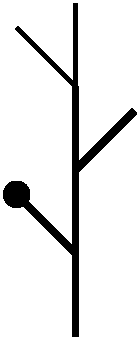
\includegraphics[height=100pt]{AcropetalSignal3}} ~
	\subfloat{\includegraphics[height=100pt]{AcropetalSignal4}} ~
	\subfloat{\includegraphics[height=100pt]{AcropetalSignal5}}
	\caption{Acropetal signal propagation}
	\label{fig:acropetalSignal}
\end{figure}

\begin{figure}[ht]
	\centering
	\subfloat{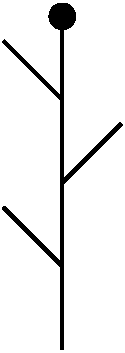
\includegraphics[height=100pt]{BasipetalSignal1}} ~
	\subfloat{\includegraphics[height=100pt]{BasipetalSignal2}} ~
	\subfloat{\includegraphics[height=100pt]{BasipetalSignal3}} ~
	\subfloat{\includegraphics[height=100pt]{BasipetalSignal4}} ~
	\subfloat{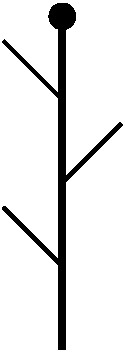
\includegraphics[height=100pt]{BasipetalSignal5}}
	\caption{Basipetal signal propagation}
	\label{fig:basipetalSignal}
\end{figure}


\subsection{Parametric \lsystems}

Symbols in parametric \lsystems can hold any number of arguments.
Arguments are floating point numbers.
Arguments can be used in interpretation definition to send values like length of line or color to interpretation routine.
Arguments can be also used in rewrite rules to determine whether rewrite symbol or not and to determine new arguments for rewritten symbols.
In context \twolsystems is also possible to get arguments from symbols in context and use them in rewrite rule.


\end{comment}


































